\section{实验与结果分析}

\subsubsection{实验设置与对比方法}

本文所有实验均在基于Ubuntu 20.04操作系统的Kaggle Notebook环境完成,硬件配置采用Kaggle提供的单张NVIDIA P100 GPU(16GB显存)和30GB RAM内存。实验模型代码基于PyTorch框架搭建,同时搭配CUDA 11.3加速库加速模型训练。

模型的网络权重的初始化采用He normal,并使用初始学习率为$1 \times 10^{-4}$的Adam优化器更新权重。每个实验都进行100轮(epoch)实验,且在每轮训练结束后在验证集上进行模型评估,保存Dice得分最高的模型权重。

本文在进行模型评估时,以Dice系数作为核心评价指标,用于衡量模模型在分割任务中预测结果与真实标签之间的重叠程度,是医学图像分割中最常用且最敏感的评估指标之一。为了更全面地反映模型性能,辅以Jaccard指数、F1分数、准确率(Accuracy)、精确率(Precision)与召回率(Recall)等多维度指标进行综合评估。

\subsection{消融和增广实验}

为了系统评估各改进模块对模型语义分割性能的影响,本研究设计了一系列消融实验,围绕模型结构、损失函数与训练策略三个层面展开。以基准U-Net模型作为对照组,逐步引入或移除关键组件,包括跳跃连接、注意力机制、数据增强策略、以及不同的损失函数组合,来观察每项设计对模型性能的独立贡献与协同增益。

所有消融与增广实验均基于ISIC 2018皮肤癌图像分割数据集进行,采用 8:2 比例划分训练集与验证集,并在固定的模型训练框架和超参数设置下进行公平比较。通过精心设计的分组实验与逐项对照分析,本节将展示各模块在模型收敛速度、最终性能、错误类型等方面的具体影响,为构建最终优化方案提供理论依据与实证支撑。

\subsubsection{基准模型性能验证}

在所有实验中,基准U-Net模型使用原始U-Net网络结构,配合混合损失函数和Adam优化器进行训练,关于损失函数和优化器的具体参数设置已在第三章阐述。此外,基准模型的训练未采用任何形式的数据增强或正则化操作,以便纯粹评估其建模能力与收敛特性。

为全面评估基准 U-Net 模型在验证集上的性能表现,图~\ref{fig:base_unet_metrics} 展示了训练过程中多个关键评估指标(包括 Dice 系数、Jaccard 指数、Accuracy、Precision、Recall、F1-Score、Specificity 及 Loss)随 epoch 变化的趋势曲线。训练曲线反映了模型收敛过程及其在训练与验证集上的性能差异,可用于分析模型的拟合能力与泛化效果。

\begin{figure}[!htbp]
    \centering
    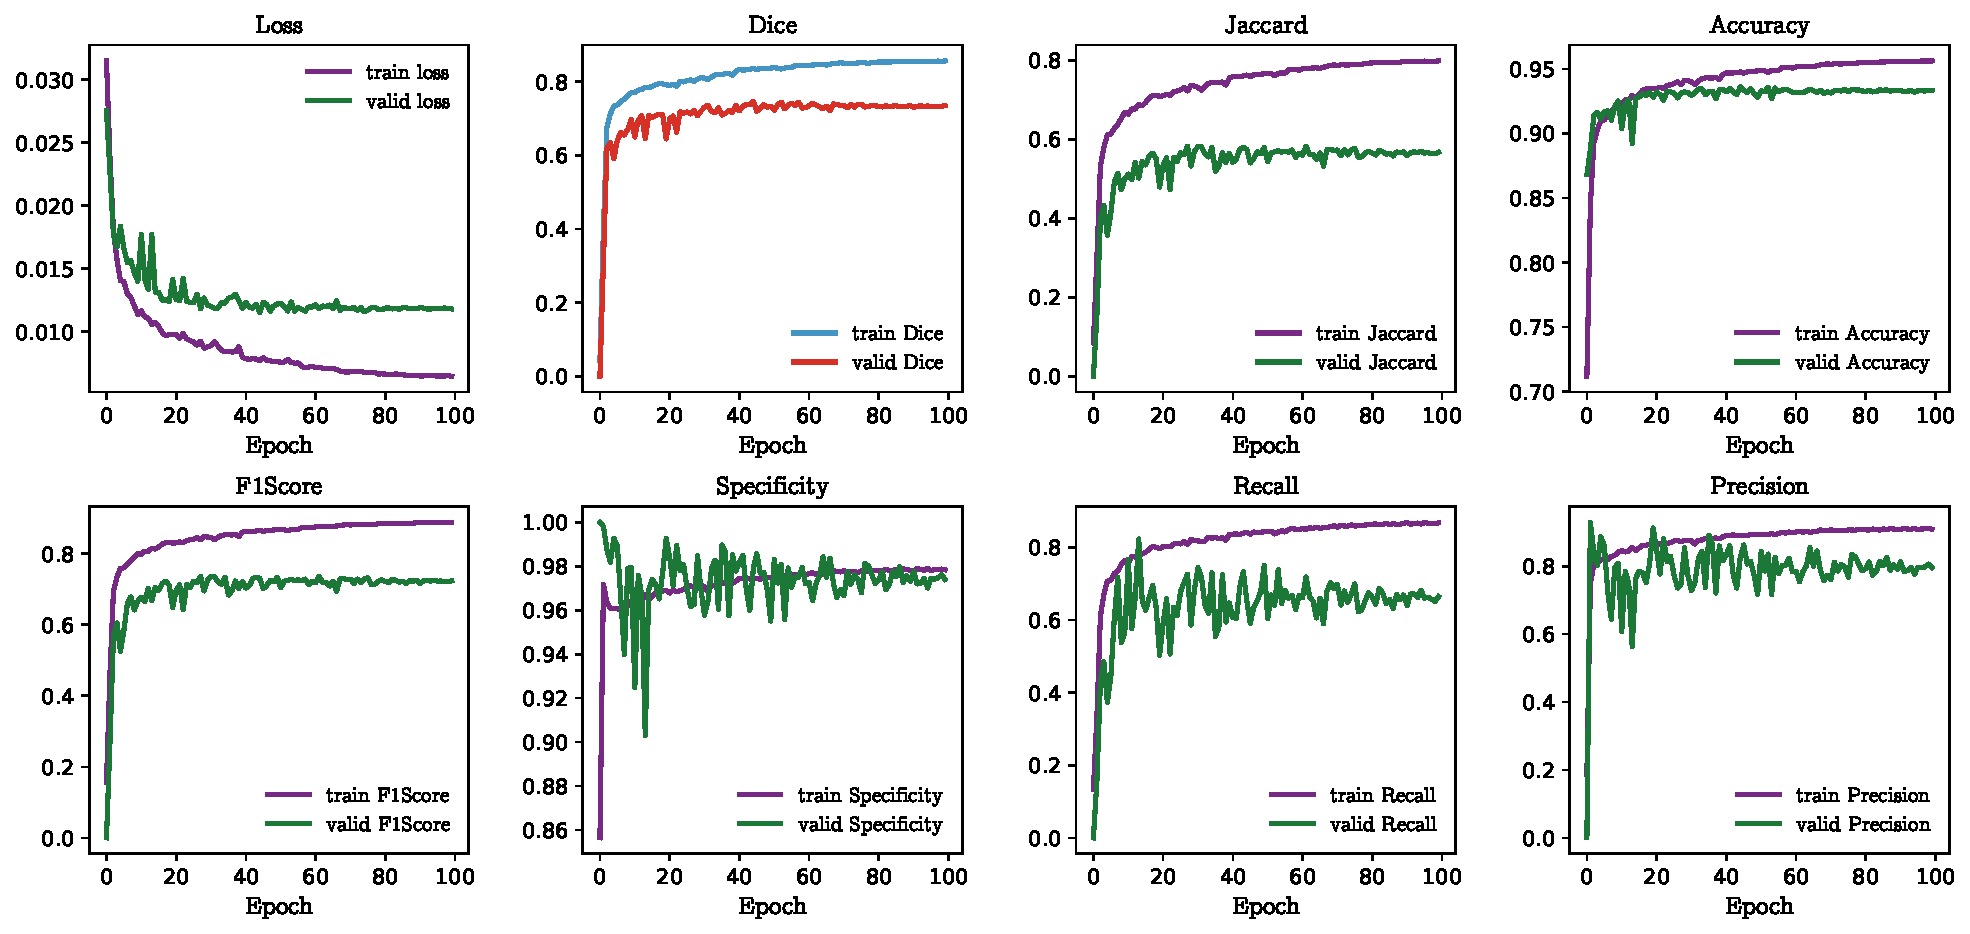
\includegraphics[width=\textwidth]{fig/base_unet_metrics.pdf}
    \caption{基准U-Net模型训练过程中的性能指标变化趋势}
    \label{fig:base_unet_metrics}
\end{figure}

表 \ref{tab:unet_epoch_compare} 对比了基线 U-Net 在验证集上的三个关键时间点——首次达到 Dice ≥ 0.70 的第 13 轮、全局最优的第 45 轮以及训练末期(最后 10 轮)——对应的主要性能指标。可以看到,模型在第 13 个 epoch 即取得 0.7077 的 Dice值 和 0.5420 的 Jaccard值,说明其收敛速度较快。随后经过 32 轮的渐进优化,Dice 进一步提升到 0.7469(+3.9 pp),Jaccard 则提升到 0.5747(+3.3 pp),而 Precision 几乎保持不变(≈ 0.826),表明网络 在保证低假阳性的同时显著减少漏检。Val-Loss 同期下降约 12 \%,与性能上升趋势一致。

此外,末 10 轮的均值与标准差(右侧一列)显示各指标波动极小(Dice σ ≈ 0.001),证明模型已进入稳定收敛区间且未出现明显过拟合。基于这一观察,本文后续将第 45 轮作为“最优性能”参考点,而第 13 轮则可作为“早期收敛效率”的对照基准,用以衡量不同改进策略在早期与最终阶段的综合效益。

\begin{table}[htbp]
    \centering
    \caption{基线U-Net模型关键Epoch验证集性能指标对比}
    \label{tab:unet_epoch_compare}
    \begin{tabular}{lcccc}
        \toprule
        指标 (val) & Epoch 13 & Epoch 45 (best) & $\Delta$ & 末10轮均值 \\
        \midrule
        Dice        & 0.7077 & \textbf{0.7469} & +3.9 pp   & 0.734 $\pm$ 0.001 \\
        Jaccard     & 0.5420 & \textbf{0.5747} & +3.3 pp   & 0.561 $\pm$ 0.002 \\
        Precision   & \textbf{0.8266} & 0.8262 & $\approx$0 & 0.822 $\pm$ 0.008 \\
        Recall      & 0.6266 & \textbf{0.6537} & +2.7 pp   & 0.645 $\pm$ 0.010 \\
        Val-Loss $\downarrow$ & 0.01312 & \textbf{0.01150} & $-12.4\%$ & 0.0117 $\pm$ 0.0002 \\
        \bottomrule
    \end{tabular}
\end{table}

\subsubsection{跳跃连接的结构消融实验}

\begin{table}[htbp]
    \centering
    \caption{Baseline U-Net 与删除跳跃连接模型在验证集上的性能对比}
    \label{tab:ablation_skip_connection}
    \begin{tabular}{lcccc}
        \toprule
        指标 & Baseline U-Net & 无跳跃连接模型 & 绝对变化 & 相对变化 \\
        \midrule
        Dice         & \textbf{0.7469} & \textbf{0.7576} & +0.0107 & +1.4\% \\
        F1           & 0.7299 & 0.7507 & +0.0208 & +2.8\% \\
        IoU / Jaccard & 0.5747 & 0.6009 & +0.0262 & +4.6\% \\
        Precision    & \textbf{0.8262} & 0.8009 & $-$0.0253 & $-$3.1\% \\
        Recall       & 0.6537 & \textbf{0.7064} & +0.0527 & +8.1\% \\
        Accuracy     & 0.9362 & 0.9352 & $-$0.0010 & $-$0.1\% \\
        Specificity  & 0.9791 & 0.9719 & $-$0.0072 & $-$0.7\% \\
        Val-Loss $\downarrow$ & 0.01150 & \textbf{0.01114} & $-$0.00036 & $-$3.1\% \\
        \bottomrule
    \end{tabular}
\end{table}

\subsubsection{损失函数的混合消融实验}

\begin{table}[htbp]
    \centering
    \caption{不同损失函数下模型性能对比(B: Baseline,D: Dice-only,C: Dice+CE)}
    \label{tab:loss_ablation}
    \begin{tabular}{lcccccc}
        \toprule
        指标(Val) & B (Ep 44) & D (Ep 99) & C (Ep 78) & $\Delta$ D$-$B & $\Delta$ C$-$B \\
        \midrule
        Dice        & 0.747 & 0.747 & \textbf{0.752} & $-$0.0004 & +0.0046 (+0.6\%) \\
        F1-score    & 0.730 & 0.734 & \textbf{0.740} & +0.004 & +0.010 \\
        Jaccard     & 0.575 & 0.580 & \textbf{0.588} & +0.005 & +0.013 \\
        Precision   & \textbf{0.826} & 0.801 & 0.776 & $-$0.025 & $-$0.050 \\
        Recall      & 0.654 & 0.677 & \textbf{0.708} & +0.024 & +0.054 \\
        Accuracy    & 0.936 & 0.935 & 0.934 & $-$0.001 & $-$0.002 \\
        Specificity & \textbf{0.979} & 0.975 & 0.969 & $-$0.004 & $-$0.010 \\
        Train$-$Val Dice & 0.089 & 0.109 & 0.113 & $\uparrow$ 0.020 & $\uparrow$ 0.024 \\
        \bottomrule
    \end{tabular}
\end{table}

\subsubsection{数据增强增广实验}

\begin{table}[htbp]
    \centering
    \caption{Baseline 与 Augment 模型在相同 Epoch (13) 下的验证集性能对比}
    \label{tab:augment_ep13}
    \begin{tabular}{lcccc}
        \toprule
        指标(Val) & Baseline (Ep 13) & Augment (Ep 13) & 绝对提升 $\Delta$ & 相对提升 \\
        \midrule
        Dice        & 0.7077 & \textbf{0.7230} & +0.0153 & +2.2\% \\
        F1-score    & 0.7030 & 0.7185 & +0.0155 & +2.2\% \\
        Jaccard     & 0.5420 & 0.5609 & +0.0189 & +3.5\% \\
        Precision   & \textbf{0.7856} & 0.7429 & $-$0.0427 & $-$5.4\% \\
        Recall      & 0.6266 & \textbf{0.6816} & +0.0550 & +8.8\% \\
        Accuracy    & 0.9264 & 0.9310 & +0.0046 & +0.5\% \\
        Specificity & 0.9667 & 0.9772 & +0.0105 & +1.1\% \\
        Val-Loss $\downarrow$ & 0.01312 & \textbf{0.01114} & $-$0.00198 & $-$15.1\% \\
        \bottomrule
    \end{tabular}
\end{table}


\subsubsection{注意力机制增广实验}

\begin{table}[htbp]
    \centering
    \caption{Baseline 与 Att-U-Net 模型在验证集上的性能对比}
    \label{tab:att_unet}
    \begin{tabular}{lcccc}
        \toprule
        指标(Val) & Baseline (Ep 44) & Att-U-Net (Ep 38) & 绝对提升 $\Delta$ & 相对提升 \\
        \midrule
        Dice        & 0.747 & \textbf{0.818} & +0.071 & +9.5\% \\
        Jaccard     & 0.575 & 0.665 & +0.091 & +15.8\% \\
        Precision   & \textbf{0.826} & 0.808 & $-$0.018 & $-$2.3\% \\
        Recall      & 0.654 & \textbf{0.791} & +0.137 & +21.0\% \\
        Accuracy    & 0.936 & 0.948 & +0.011 & +1.2\% \\
        Loss $\downarrow$ & 0.0115 & \textbf{0.0105} & $-$0.0010 & $-$8.8\% \\
        \bottomrule
    \end{tabular}
\end{table}

\subsubsection{最终模型}

\begin{table}[htbp]
    \centering
    \caption{融合改进模型(Att + Aug + Hybrid Loss)与 Baseline 性能对比}
    \label{tab:final_model}
    \begin{tabular}{lcccc}
        \toprule
        验证指标 & Baseline ($\sim$Ep 44) & Att + Aug + Hybrid & $\Delta$ & 相对提升 \\
        \midrule
        Dice        & 0.747 & \textbf{0.829} & +0.082 & +11\% \\
        F1-score    & 0.730 & \textbf{0.814} & +0.084 & +11.5\% \\
        Jaccard     & 0.575 & \textbf{0.687} & +0.112 & +19.5\% \\
        Precision   & 0.826 & \textbf{0.843} & +0.017 & +2.1\% \\
        Recall      & 0.654 & \textbf{0.787} & +0.133 & +20.3\% \\
        Accuracy    & 0.936 & \textbf{0.950} & +0.014 & +1.5\% \\
        Specificity & \textbf{0.979} & 0.977 & $-$0.002 & $-$0.2\% \\
        Val-Loss $\downarrow$ & 0.0115 & \textbf{0.00885} & $-$0.00265 & $-$23\% \\
        \bottomrule
    \end{tabular}
\end{table}

\subsection{泛化性测试}
%在不同医学图像模态(如CT、MRI)和不同器官分割任务中测试改进方法的泛化能力。
%分析模型在不同任务中的表现,验证其在多种场景下的适用性和鲁棒性。


\subsection{方法局限性讨论}
%研究在不同大小的训练数据集下,改进方法的模型性能变化。
%分析模型在小数据集和大数据集上的表现差异,评估其对数据量的敏感性和鲁棒性。
